\subsection{Linear regression with forward selection}
When predicting the CHD using linear regression we have tried using both all the attributes, and using the attributes found using Forward Selection, this is the results for Linear regression without feature selection :
\begin{itemize}
\item Training error: 0.172
\item Test error: 0.183
\item $R^{2}$ Train: 0.24
\item $R^{2}$ Test: 0.19
\end{itemize}
And this is for Linear regressions with feature selection:
\begin{itemize}
\item Training error: 0.174
\item Test error: 0.186
\item $R^{2}$ Train: 0.231
\item $R^{2}$ Test: 0.177
\end{itemize}
When using feature selection, the produced values are almost identical to the ones when using all attributes, which could indicate that our feature selection is good.

The feature selection gives the following output:
\begin{figure}[H]
\centering
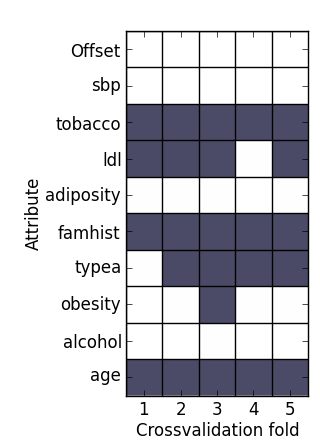
\includegraphics[width=4cm, keepaspectratio=true]{pictures/cv_fold.png}
\caption{Feature selection}
\label{featureSelection}
\end{figure}
From the original list of 9 attributes, only 5 attributes are needed to maintain the performance of the model while making the model more simple. These attributes are:
\begin{itemize}
\item Tobacco
\item ldl
\item famhist
\item typeA
\item Age
\end{itemize}



\subsubsection{Predicting using linear regression}
As of now, the model has an $R^{2}$ of around 0.2 which is not that good. this results in the following prediction from our model:
\begin{figure}[H]
\centering
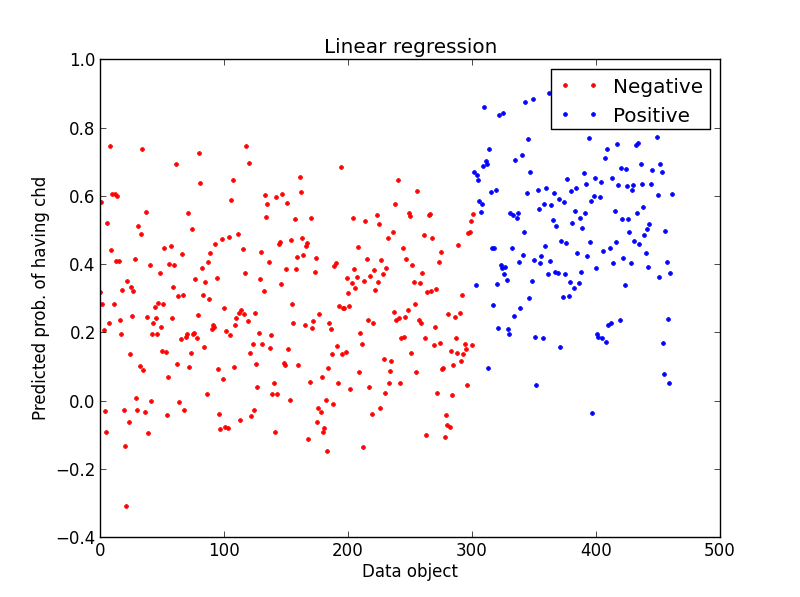
\includegraphics[width=12cm, keepaspectratio=true]{pictures/linearPrediction.png}
\caption{Prediction of our linear regression model}
\label{linearPrediction}
\end{figure}
The data is sorted, so it is easier to see the switch from negative CHD to positive.

The plot of the prediction shows that the model is definately not doing an excellent job predicting whether a person has CHD or not, however it is possible too see a pattern, that most negative CHD cases are < 0.5, and most positive CHD cases are > 0.5

The overall misclassification rate using linear regression is 35.7\%

In the following section we will discuss if model transformation could possibly enhance the model
\subsubsection{Residual error plot}
A plot of the residual error vs the attribute shows the following:
\begin{figure}[H]
\centering
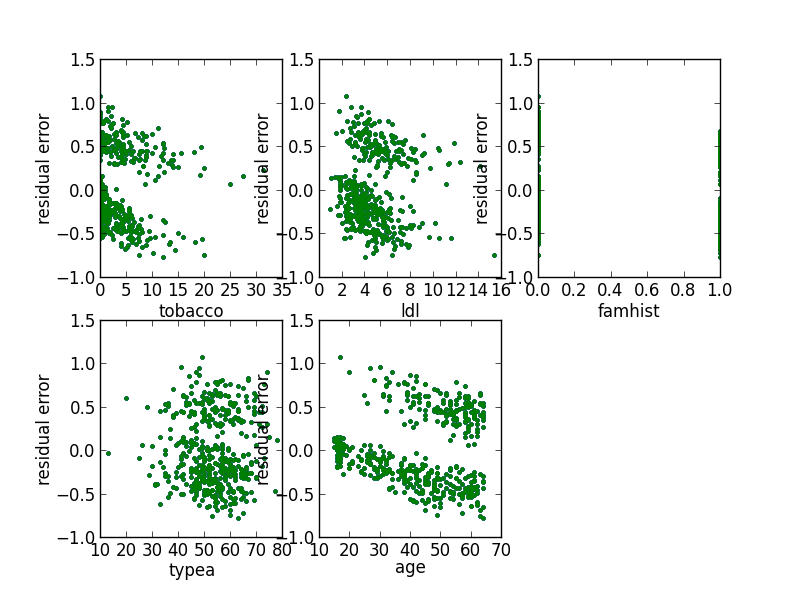
\includegraphics[width=12cm, keepaspectratio=true]{pictures/residual_error.png}
\caption{Plot of residual error vs the attribute}
\label{residualError}
\end{figure}
A good residual error vs attribute plot would be randomly distibuted along the horizontal axis. Looking at the plot, this is not the case for the plotted attributes. This could indicate that a transformation of the attributes could enhance the model.